\documentclass[12pt,letterpaper]{exam}
\usepackage[lmargin=1in,rmargin=1in,tmargin=1in,bmargin=1in]{geometry}
\usepackage{../style/exams}

% -------------------
% Course & Exam Information
% -------------------
\newcommand{\course}{MAT 108: Exam 3}
\renewcommand{\term}{Fall -- 2022}
\newcommand{\examdate}{12/15/2022}
\newcommand{\timelimit}{85 Minutes}

\setbool{hideans}{true} % Student: True; Instructor: False

% -------------------
% Content
% -------------------
\begin{document}

\examtitle
\instructions{Write your name on the appropriate line on the exam cover sheet. This exam contains \numpages\ pages (including this cover page) and \numquestions\ questions. Check that you have every page of the exam. Answer the questions in the spaces provided on the question sheets. Be sure to answer every part of each question and show all your work. If you run out of room for an answer, continue on the back of the page --- being sure to indicate the problem number.} 
\scores
\bottomline
\newpage

% ---------
% Questions
% ---------
\begin{questions}

% Question 1
\newpage
\question[10] Define the following vectors:
	\[
	\mathbf{u}= \begin{pmatrix} 2 \\ -1 \\ 0 \\ -3 \end{pmatrix} \qquad
	\mathbf{v}= \begin{pmatrix} 5 \\ 2 \\ -1 \\ 4 \end{pmatrix}
	\]
Showing all your work, compute the following:
	\begin{enumerate}[(a)]
	\item $-3 \mathbf{u}$
	\item $\mathbf{v} - \mathbf{u}$
	\item $\mathbf{u} \cdot \mathbf{v}$
	\end{enumerate}



% Question 2
\newpage
\question[10] Define the following matrices:
	\[
	A= \begin{pmatrix} 1 & -1 \\ 0 & 4 \end{pmatrix} \qquad
	B= \begin{pmatrix} -2 & 0 & 1 \\ 3 & -1 & 5 \end{pmatrix} \qquad
	C= \begin{pmatrix} 6 & 1 \\ -2 & 3 \end{pmatrix}
	\]

\begin{enumerate}[(a)]
\item Compute $B^T$.
\item Showing all your work, compute $5A$.
\item Showing all your work, compute $A - C$.
\item Only one of the possible matrix products $AB$ and $BA$ is defined. For the one which is defined, showing all your work, compute that product. 
\end{enumerate}



% Question 3
\newpage
\question[10] Consider the following system of linear equations:
	\[
	\begin{aligned}
	5x_1 - 3x_2 + 4x_3 - x_4= 12 \\
	x_1 + 10x_2 + 9x_4= 10 \\
	6x_1 - x_2 + 2x_3 + x_4= -6
	\end{aligned}
	\]

\begin{enumerate}[(a)]
\item Find the coefficient matrix for this system of equations. 
\item Find the solution vector for this system of equations.
\item Find the augmented matrix for this system of equations. 
\end{enumerate}



% Question 4
\newpage
\question[10] Below is an augmented matrix corresponding to a system of linear equations in reduced-row echelon form. If there were solution(s) to the system of equations, find them. If not, explain why. 
	\[
	\begin{pmatrix}
	1 & 0 & 0 & 5 \\
	0 & 1 & 0 & -6 \\
	0 & 0 & 1 & 7
	\end{pmatrix}	
	\]



% Question 5
\newpage
\question[10] Below is an augmented matrix corresponding to a system of linear equations in reduced-row echelon form. If there were solution(s) to the system of equations, find them. If not, explain why. 
	\[
	\begin{pmatrix}
	1 & 0 & 0 & 0 & 6 \\
	0 & 1 & 0 & 0 & 1 \\
	0 & 0 & 1 & 0 & -4 \\
	0 & 0 & 0 & 0 & 1 
	\end{pmatrix}	
	\]



% Question 6
\newpage
\question[10] Below is an augmented matrix corresponding to a system of linear equations in reduced-row echelon form. If there were solution(s) to the system of equations, find them. If not, explain why. 
	\[
	\begin{pmatrix}
	1 & 0 & 0 & -5 \\
	0 & 1 & -3 & 8 \\
	0 & 0 & 0 & 0
	\end{pmatrix}	
	\]



% Question 7
\newpage
\question[10] Consider the feasible set given below:
	\[
	\fbox{
	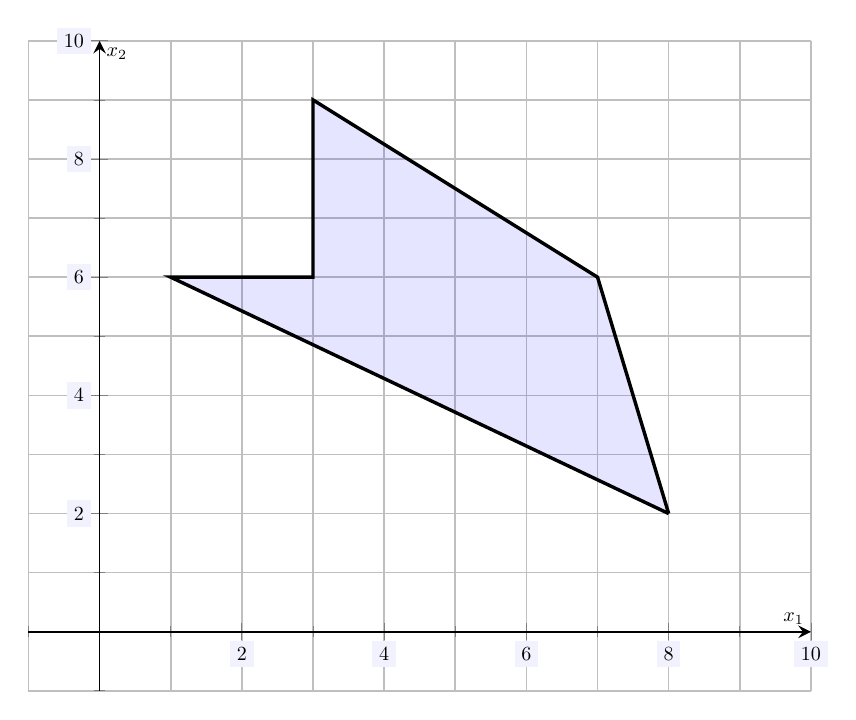
\begin{tikzpicture}[scale=1.45,every node/.style={scale=0.5}]
	\begin{axis}[
	grid=both,
	axis lines=middle,
	ticklabel style={fill=blue!5!white},
	xmin= -1, xmax=10,
	ymin= -1, ymax=10,
	xtick={0,2,4,6,8,10},
	ytick={0,2,4,6,8,10},
	minor tick = {-1,0,1,...,10},
	xlabel=\(x_1\),ylabel=\(x_2\),
	]
	\draw[line width=0.01cm,fill= blue,opacity=0.1] (8,2) -- (7,6) -- (3,9) -- (3,6) -- (1,6) -- (8,2);
	\draw[line width=0.03cm] (8,2) -- (7,6) -- (3,9) -- (3,6) -- (1,6) -- (8,2);
	\end{axis}
	\end{tikzpicture}
	}
	\]
Fully explaining your reasoning and showing all your work, find the maximum and minimum value of $z= 6x_1 - 5x_2$ on this feasible set. 

	

% Question 8
\newpage
\question[10] Find the initial simplex tableau corresponding to the maximization problem shown below:
	\[
	\begin{aligned}
	\max z= 4.3x_1 \,+ &\,5.7x_2 - 7.1x_3 - 5.6 x_4 \\
	6.9x_1 - 3.3x_2 &+ 7.9x_4 \leq 10.3 \\
	2.4x_1 - 5.8x_2 &+ 7.3x_3 \leq 14.3 \\
	8.4x_1 - 9.2x_2 \,+\, &1.8x_3 - 3.1x_4 \geq -10.8 \\
	x_1, x_2, &\, x_3, x_4 \geq 0
	\end{aligned}
	\]



% Question 9
\newpage
\question[10] Below is the initial simplex tableau corresponding to some maximization problem. Find the corresponding maximization problem. \par
	\begin{table}[!ht]
	\centering
	\begin{tabular}{rrrrrrr}
	$4$ & $5$ & $1$ & $0$ & $0$ & $0$ & $6$ \\
	$-6$ & $2$ & $0$ & $1$ & $0$ & $0$ & $8$ \\
	$1$ & $-1$ & $0$ & $0$ & $1$ & $0$ & $9$ \\
	$-1$ & $5$ & $0$ & $0$ & $0$ & $1$ & $4$ \\
	$-6$ & $8$ & $0$ & $0$ & $0$ & $0$ & $0$
	\end{tabular}
	\end{table}



% Question 10
\newpage
\question[10] Below is the final simplex tableau corresponding to some maximization problem. Find the solution to the original optimization problem. \par
	\begin{table}[!ht]
	\centering
	\begin{tabular}{rrrrrrr}
	$0.54$ & $0.29$ & $1$ & $0$ & $0.10$ & $-0.02$ & $11.37$ \\
	$2.37$ & $1.23$ & $0$ & $1$ & $-0.07$ & $0.14$ & $21.67$ \\
	$24.77$ & $20.45$ & $0$ & $0$& $0.10$ & $1.48$ & $341.7$
	\end{tabular}
	\end{table}



% Question 11
\newpage
\question[10] Find the dual problem for the following minimization problem:
	\[
	\begin{aligned}
	\min w= 5y_1 &- 7y_2 + 6y_3 \\
	y_1 - y_2 &+ y_3 \geq 6 \\
	-4y_1 + 3y_2 &- y_3 \geq 10 \\
	6y_1 + y_2 &+ 4y_3 \geq 3 \\
	y_1, y_2, \,&y_3 \geq 0
	\end{aligned}
	\]



% Question 12
\newpage
\question[10] Find the initial simplex tableau for the following maximization problem:
	\[
	\begin{aligned}
	\max z= x_1 - &2x_3 + 3x_3 \\
	4x_1 - 3x_2 &+ x_3 \geq 10 \\
	x_1 - x_2 + &6x_3 \leq 15 \\
	3x_1 \,+ &\,8x_2 \leq 12 \\
	x_1 - x_2 \,-\, &4x_3 \geq -20 \\
	x_1, x_2, \,&x_3 \geq 0 
	\end{aligned}
	\]
	















\end{questions}
\end{document}